\section{Introduction}

% 360 degree videos are important
360-degree videos are coming to age, which has been driven by content
providers (\eg CNN, New York Times) serving more immersive content (\eg 
NBC broadcasting the 2018 Winter Olympics in VR~\cite{NBC_olympic_360}), as well as 
by more application platforms~\cite{google_developers,facebook360} and 
devices (\eg Samsung smartphone headset~\cite{SUMSUNG_HEADSET}).
However, streaming 360-degree videos to mobile devices through wireless
networks remains a substantial challenge.

% why it's challenging
To provide true immersive experience, the 360-degree video must be streamed
in high resolution and within a small bounded delay.

\begin{packeditemize}
% low delay
\item {\em Stringent delay constraint:} 

To prevent simulator sickness \cite{Simulator_Sickness} and to provide good Quality of Experience (QoE), the vendors of HeadMounted Displays (HMD) recommend that the video systems
react to head movements as fast as the HMD refresh rate, i.e., frames per second (fps).
Since fps of state-of-the-art HMDs is 120 Hz,
the whole system should react in less than 10 ms. These stringent delay constraints render many traditional streaming 
protocols (\eg~\cite{MPEG-DASH},~\cite{FESTIVE}) insufficient.

%\jc{reword the last sentence. what's "application round-trip latency"? why "sickness" is caused by some "refresh rate"?} These stringent delay constraints render many traditional streaming  protocols (\eg~\cite{??,??}) insufficient.

% high bandwidth
\item {\em High-bandwidth consumption:}
Moreover, 360-degree videos require high bandwidth to stream videos in
high resolution, ideally, over the whole 360-degree sphere; \eg the 
bitrate of an 8K 360-degree video feed encoded at a frame rate of 60 fps
(frames per second) with HEVC~\cite{HEVC} is $\sim$100Mbps. According to
OpenSignal~\cite{opensignal}, almost a half of the 77 surveyed 
countries in 2017 over the world only have access to 4G cellular 
networks of 10-25 Mbps.
\end{packeditemize}

% fov-aware streaming & problems
One of the common approaches to addressing this challenge is that, 
instead of streaming all video content simultaneously, one can stream
only the video content in and around the viewer's field of view (FOV),
or prioritize data in those FOV regions over non-FOV regions. This 
FOV-aware approach has attracted great attention in recent 
years~\cite{Viewport-adaptive,360ProbDASH,Adaptive_Streaming_Framework,Two-tier,Omnidirectional_Video_over_HTTP,Furion}, 
leading to many strategies that adapt application-level parameters, \eg 
encoding bitrate, to allocate bandwidth so as to ensure good quality of
content in the FOV regions. However, these application-level strategies 
do not directly optimize for the delay constraints. This is because 
they run on top of existing transport protocols that are unaware of FOVs
and thus fail to leverage the fact that data packets may have different
inherent priority depending on whether the carried video data belong to
FOV region.

% custom transport protocols & problems
On the other hand, there have been proposals of custom transport 
protocols for streaming delay-sensitive videos~\cite{MPMTP,CMT-VR,ADMIT}. 
Unfortunately, they have so far focused on traditional video content, 
as opposed to 360-degree videos. So the opportunities of developing a 
custom transport protocol for 360-degree video streaming remain untapped.
In particular, it remains unclear how to leverage the knowledge of FOV
to adapt transport-level actions, \eg packet scheduling and setting of 
the redundancy level in error correction code.

% our solution
In this paper, we propose {\em Dante}, an FOV-aware transport protocol
for 360-degree video streaming. Figure. 2 puts Dante into the perspective
of previous efforts. At the core of Dante are two ideas. First, like 
other video-specific custom streaming protocols, Dante does not enforce
total reliability which are likely to be blocked by re-transmissions, 
Dante uses Forward Error Correction (FEC) to recover data losses 
without retransmissions, thus significantly reducing the streaming delay.
While these protocols might cause small fraction of missing frames 
(except key frames for which we do apply retransmission to ensure 
reliability), our evaluation shows that its impact on video quality is 
negligible, even under highly lossy network connections. 
Second, Dante prioritizes FOV regions by using more FEC redundancy to 
send data packets belonging to FOV regions (predicted by the 
video player). This effectively gives packets in FOV regions more 
bandwidth, higher reliability, and more chance to meet the streaming 
delay constraint.

We use two video sequences downloaded from Youtube as our dataset to evaluate the performance of Dante. The experimental results show that Dante improves video PSNR over current video transport protocols by 20\% to 30\%.

%\jc{need a para to summarize the key results: 
%we use what dataset to evaluate the performance of Dante and compares it against what baseline.  the experimental results show that Dante improves what metrics over  what baselines by how much}













%%% OLD INTRO
\begin{comment}
	
With the promise of immersive visual experience, 360-degree videos are widely applied in sports field, social field~\cite{facebook360}, and apps development field~\cite{google_developers}, etc. Meanwhile, it has been well deployed across mainstream content providers such as NBC (who broadcast the 2018 winter Olympics in VR), news outlets, such as CNN, New York Times, and user-generated content platform such as Youtube and Facebooks.
However, some significant challenges still remain as the major bottlenecks for 360-degree technologies, even worse in mobile scenarios.

The bottleneck can be summarized as that wireless links are characterized by limited resources and error-prone problems, while 360-degree video streaming
is characterized by bandwidth intensiveness and delay sensitivity.

%% One aspect of technological challenges stems from stringent delay and high bandwidth requirement. 
%% To prevent simulator sickness~\cite{Simulator_Sickness}, the whole system needs to react as fast as the refresh rate of Head-mounted Display(HMD), such as 120 Hz, in other words, this means application round-trip latency is supposed to be less than 10ms for imperceptible Motion-To-Photon(MTP) latency. Such the rigorous delay constraint prevents the implementation of those traditional protocols based on feedback and retransmissions.
For example, application round-trip latency is supposed to be less than 10ms for imperceptible Motion-To-Photon(MTP) latency in order to prevent simulator sickness~\cite{Simulator_Sickness}, due to the refresh rate of Head-mounted Display(HMD), such as 120 Hz. Such the rigorous delay constraint prevents the implementation of those traditional protocols based on feedback and retransmissions.

Meanwhile, 360-degree videos have the requirement of high bandwidth in order to enable immersive experience. The bit-rate of 8K 360-degree videos at 60 fps encoded using High Efficiency Video Coding (HEVC)~\cite{HEVC} is around 100 Mbps. However, according to OpenSignal~\cite{opensignal}, covering 77 countries in the world, almost a half of countries have access to 4G cellular network with only 10-25 Mbps speed in 2017. Obviously, it's not available and practical to deploy 360-degree videos service in mobile scenarios.    

Currently, based on the observation that only the FOV region of video is only perceived by user anytime, FOV-aware tile-based streaming~\cite{Viewport-adaptive}\cite{360ProbDASH}\cite{Adaptive_Streaming_Framework} \cite{Two-tier}\cite{Omnidirectional_Video_over_HTTP}\cite{Furion}, a scheme of application layer, is proposed to mitigate the requirement of bandwidth and delay, due to the introduction of FOV-aware bit-rate adaptation and video segment prefeatching. However, it achieves poor performance over wireless links, featured by limited bandwidth and error-prone characteristic, because the most advanced transport protocols it uses fail to consider FOV, for example, their reliability schemes of transport layer fail to consider FOV.     

In this paper, we propose Dante, as depicted in Figure 1, an application-layer 360-degree video protocol.
In this proposed Dante, instead of only transmissions, FEC is adopted to strengthen reliability scheme, which can recover data loss over wireless lossy links, mitigating video quality degradation. 
And the core of the reliability scheme is an FEC adaptation, which is FOV-aware and performs hierarchical error protection on different region of the video, spatially.

%We first design a FOV-aware video distortion model, and from the perspective of reliability schemes, design an FOV-aware FEC parameter adjusting algorithm based on that model to achieve low latency. Furthermore, we design an FOV-aware packet scheduling algorithm, which preferentially allocates better bandwidth for more crucial data, and thus boosting video quality and achieving graceful degradation even under poor network condition.
\end{comment}

\begin{figure}[ht]
	\centering
	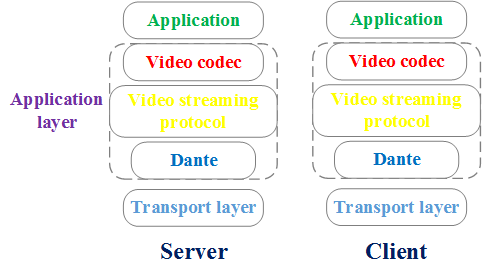
\includegraphics[scale=0.4]{paper_figs/stack_dante.png}
	\caption{Illustration Of Dante}
	\label{paper_figs:pathdemo}
\end{figure}

\begin{figure}[ht]
	\centering
	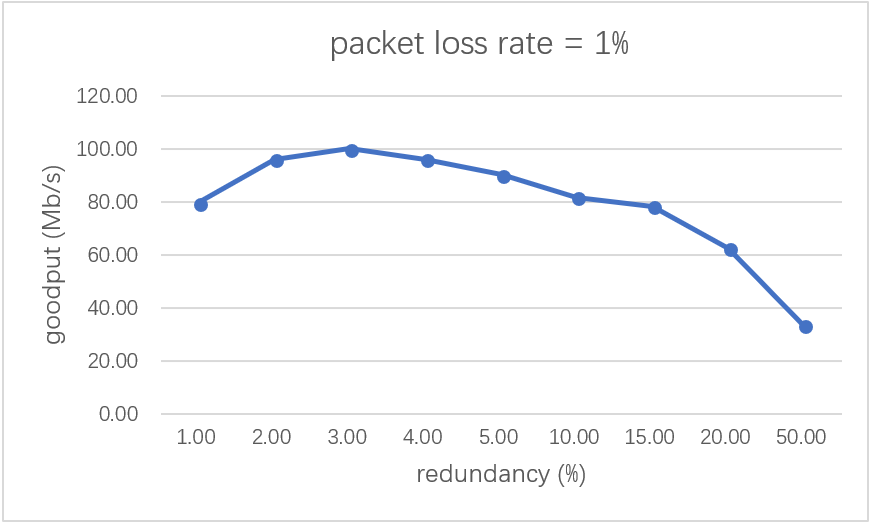
\includegraphics[scale=0.25]{paper_figs/tradeoff_only_goodput.png}
	\caption{The Goodput When Increasing The FEC Redundancy}
	\label{paper_figs:pathdemo}
\end{figure}

